\documentclass{../c-lecture}

\subtitle{Pointers \& Dynamic Memory}

\begin{document}

\begin{frame}
  \titlepage{}
\end{frame}
\begin{frame}
  \frametitle{Outline}
  \tableofcontents{}
\end{frame}

\section{Introduction}

\begin{frame}[fragile]
  \frametitle{Pointer: Reference to Memory}
  \begin{itemize}
    \item Pointer is a variable that
    \begin{itemize}
      \item
        Contains the \textit{\color{Orange} address} of another variable
    \end{itemize}
    \item Pointer \textit{\color{LimeGreen} refers} to an address
    \item Examples
    \begin{minted}[bgcolor=Black]{c}
int i;
int *pi;
i = 20;
pi = &i;
    \end{minted}
  \end{itemize}
\end{frame}

\begin{frame}[fragile]
  \frametitle{Pointer: Declaration and Initialization}
  \begin{itemize}
    \item
      {\color{Orange}<type>}*
      {\color{LimeGreen}<identifier>};
    \item Example
    \begin{minted}[bgcolor=Black]{c}
int i, *pi;
pi = &i;
float f;
float *pf = &f;
    \end{minted}
  \end{itemize}
\end{frame}

\begin{frame}[fragile]
  \frametitle{Value of referred memory by a pointer}
  \begin{minted}[bgcolor=Black]{c}
int *pi, *pj, i, j;
  \end{minted}
  \begin{itemize}
    \item
      \textit{\color{YellowOrange} pi} variable contains the memory address
    \begin{itemize}
      \item
        If you assign a value to it:
        \mintinline{c}|pi = &i;|
      \begin{itemize}
        \item The address is saved in \textit{\color{Cyan} pi}
      \end{itemize}
      \item If you read it: \mintinline{c}|pj = pi;|
      \begin{itemize}
        \item
          The address is copied from \textit{\color{Cyan} pi} from
          \textit{\color{LimeGreen} pj}
      \end{itemize}
    \end{itemize}
  \end{itemize}
\end{frame}

\begin{frame}
  \begin{itemize}
    \item
      \textit{\color{YellowOrange} *pi} is the value of referred memory

    \begin{itemize}
      \item If you read it: \mintinline{c}|j = *pi;|
      \begin{itemize}
        \item
          The \textbf{\color{Cyan} value in the referred address} is
          read from pi

      \end{itemize}
      \item
        If you assign a value to it: \mintinline{c}|*pj = i;|

      \begin{itemize}
        \item
          The value is saved in the
          \textbf{\color{Cyan} referred address}
      \end{itemize}
    \end{itemize}
  \end{itemize}
\end{frame}

\begin{frame}[fragile]
  \frametitle{Using Pointers: Example}
  \begin{minted}[bgcolor=Black]{c}
int i = 10, j;
/* address of i is 100, value of i is 10 */
/* address of j is 200, value of j is ?? */
int *pi;
/* address of pi is 300, value of pi is ?? */
pi = &i;
/* address of pi is 300, value of pi is 100 */
j = *pi;
/* address of j is 200, value of j is 10 */
*pi = 20;
/* address of pi is 300, value of pi is 100 */
/* address of i is 100, value of i is 20 */
  \end{minted}
\end{frame}

\begin{frame}[fragile]
  \frametitle{Using Pointers: Example}
  \begin{minted}[bgcolor=Black]{c}
double d1, d2, *pda, *pdb;
d1 = 10;
d2 = 20;
pda = &d1;
pdb = &d1;
*pda = 15;
d2 = d2 + *pdb;
printf("d2 = %f\n", d2); // d2 = 35.0
  \end{minted}
\end{frame}

\begin{frame}
  \frametitle{Pointer: Reference to Memory}
  \begin{itemize}
    \item Pointer variable contains an address
    \item There is a special address
    \mint{c}|NULL|
    \item We can \textsc{\color{RubineRed} Not}
    \begin{itemize}
      \item Read any value from \mintinline{c}|NULL|
      \item Write any value to \mintinline{c}|NULL|
    \end{itemize}
    \item If you try to read/write \textrightarrow Run time error
    \item \mintinline{c}|NULL| is usually used
    \begin{itemize}
      \item For pointer initialization
      \item Check some conditions
    \end{itemize}
  \end{itemize}
\end{frame}

\section{Pointers and Functions}

\begin{frame}[fragile]
  \frametitle{Call by value}
  \begin{minted}[bgcolor=Black]{c}
void func(int y){
  y = 0;
}

void main(void){
  int x = 100;
  func(x);
  printf("%d", x); // 100 not 0
}
  \end{minted}
  \begin{itemize}
    \item Call by value
    \begin{itemize}
      \item The \textit{\color{YellowOrange} value} of the x is copied to y
      \item By changing y, x is \textsc{\color{RubineRed} not} changed
    \end{itemize}
  \end{itemize}
\end{frame}

\begin{frame}[fragile]
  \frametitle{Call by reference}
  \begin{itemize}
    \item Call by reference
    \begin{itemize}
      \item
        The value of variable is \textsc{\color{RubineRed}not} copied to
        function
      \item
        If function changes the input parameter \textrightarrow the variable passed to
        the input is changed
      \item Is implemented by pointers in C
    \end{itemize}
  \end{itemize}
  \begin{minted}[bgcolor=Black]{c}
void func(int *y){
  *y = 0;
}
void main(void){
  int x = 100;
  func(&x);
  printf("%d", x); // 0 ☺️
}
  \end{minted}
\end{frame}

\begin{frame}[fragile]
  \frametitle{Pointers in Functions}
  \begin{minted}[bgcolor=Black]{c}
void add(double a, double b, double *res) {
  *res = a + b;
  return;
}

int main(void) {
  double d1 = 10.1, d2 = 20.2;
  double result = 0;
  add(d1, d2, &result);
  printf("%lf\n", result); // 30.3
  return 0;
}
  \end{minted}
\end{frame}

\begin{frame}[fragile]
  \frametitle{What happen?}
  \begin{itemize}
    \mint{c}|double result = 0;|
    \item The address of result is 100, value of result is 0
    \mint{c}|add(d1, d2, &result);|
    \item
      \textit{\color{YellowOrange} Value} of d1,
      \textit{\color{YellowOrange} Value} of d2 and the
      \textit{\color{LimeGreen} address} of result is
      \textsc{\color{Purple} copied} to add

    \mint{c}|add(double a, double b, double *res)|
    \item
      Value of a is the value of d1, value of b is the value of d2 and value
      of \textit{\color{LimeGreen} res is 100} and the
      \textit{\color{YellowOrange} value of *res is 0}
  \end{itemize}
\end{frame}

\begin{frame}[fragile]
  \begin{itemize}
    \mint{c}|*res = a + b;|
    \item
      Value of a is added to b and output is saved in
      \textbf{\color{YellowOrange} the referred address by res (100)}
    \item
      But the 100 is the address of \textbf{\color{Cyan} result}.
      Therefore the value is saved in memory location result
  \end{itemize}
\end{frame}

\begin{frame}[fragile]
  \frametitle{Swap function ❌}
  \scriptsize
  \begin{minted}[bgcolor=Black]{c}
void swap(double a, double b) {
  double temp;
  temp = a;
  a = b;
  b = temp;
  return;
}

int main(void){
  double d1 = 10.1, d2 = 20.2;
  printf("d1 = %lf, d2 = %lf\n", d1, d2); // d1 = 10.1, d2 = 20.2
  swap(d1, d2);
  printf("d1 = %lf, d2 = %lf\n", d1, d2); // d1 = 10.1, d2 = 20.2
  return 0;
}
  \end{minted}
\end{frame}

\begin{frame}[fragile]
  \frametitle{Swap function ✅}
  \scriptsize
  \begin{minted}[bgcolor=Black]{c}
void swap(double *a, double *b) {
  double temp;
  temp = *a;
  *a = *b;
  *b = temp;
  return;
}

void main(void) {
  double d1 = 10.1, d2 = 20.2;
  printf("d1 = %lf, d2 = %lf\n", d1, d2); // d1 = 10.1, d2 = 20.1
  swap(&d1, &d2);
  printf("d1 = %lf, d2 = %lf\n", d1, d2); // d1 = 20.2, d2 = 10.1
}
  \end{minted}
\end{frame}

\begin{frame}
  \frametitle{Pointer as the function output}
  \begin{itemize}
    \item Functions can return a pointer as output
    \item
      But, the address pointed by the pointer must be valid after the function
      finishes

    \begin{itemize}
      \item The pointed variable must be exist
      \item
        It must \textsc{\color{RubineRed} not} be
        \textit{\color{Orange} automatic local variable} of the function

      \item
        It can be static local variable, global variable, or the input parameter

    \end{itemize}
  \end{itemize}
\end{frame}

\begin{frame}[fragile]
  \frametitle{Pointer as the function output}
  \begin{minted}[bgcolor=Black]{c}
int gi;

int *func_a(void) {
  return &gi;
}

float *func_b(void) {
  static float x;
  return &x;
}
  \end{minted}
\end{frame}

\section{Pointers and Arrays}

\begin{frame}[fragile]
  \frametitle{Operations on Pointers}
  \begin{itemize}
    \item Arithmetic
    \begin{block}{}
      \textit{\color{YellowOrange}<pointer>} - or +
      \textit{\color{YellowOrange}<integer>} (or
      \textit{\color{YellowOrange}<pointer>} -= or +=
      \textit{\color{YellowOrange}<integer>})

      \textit{\color{YellowOrange}<pointer>} -
      \textit{\color{YellowOrange}<pointer>} (they must be the same
      type)

      \textit{\color{YellowOrange}<pointer>}++ or
      \textit{\color{YellowOrange}<pointer>}--
    \end{block}
    \item Comparison between pointers
    \begin{minted}[bgcolor=Black]{c}
int arr[20];
int *pi, *pj, i;
pi = &arr[10];
pj = &arr[15];
i = pj - pi; // i = 5
i = pi - pj; // i = -5
if(pi < pj) // if is True
if(pi == pj) // if is False
    \end{minted}
  \end{itemize}
\end{frame}

\begin{frame}[fragile]
  \frametitle{Operations on Pointers Examples}
  \begin{minted}[bgcolor=Black]{c}
int *pi, *pj, *pk, i, j, k;
char *pa, *pb, *pc, a, b, c;
pi = &i;
pj = pi + 2;
pk = pj + 2;
pa = &a;
pb = pa + 2;

i = pj - pi; // i = 2
j = pb - pa; // j = 2
k = pk - pi; // k = 4

pi = pj + pk; // compile error: No + for 2 pointers
pc = pi; // compile error: Different types
i = pa – pi; // compile error: Different ptr types
  \end{minted}
\end{frame}

\begin{frame}[fragile]
  \frametitle{Array \& Pointers}
  \begin{itemize}
    \item Pointer can refer to each element in an array
    \begin{minted}[bgcolor=Black]{c}
int a[20];
int *pa;
pa = &a[10]; // pa refers to element 10
a[11] = *pa; // value of pa is saved in element 11
    \end{minted}
    \item The name of array is the pointer to the first element
    \begin{minted}[bgcolor=Black]{c}
pa = a; // pa refers to element 0
pa = &a[0];// pa refers to element 0
    \end{minted}
  \end{itemize}
\end{frame}

\begin{frame}[fragile]
  \frametitle{Array \& Pointers}
  \begin{minted}[bgcolor=Black]{c}
int a[50];
int *pa;
pa = a;
  \end{minted}
  \begin{itemize}
    \item If address a = 100
    \begin{itemize}
      \item pa = 100
    \end{itemize}
    \item pa+1 points to a[1]
    \begin{itemize}
      \item pa + 1 = 104
    \end{itemize}
    \item pa + 2 points to a[2]
    \begin{itemize}
      \item pa + 2 = 108
    \end{itemize}
  \end{itemize}
  \begin{block}{}
    \textit{\color{YellowOrange}p[i]}
    \textit{\color{LimeGreen}is equal to}
    \textit{\color{Yellow}*(p + i)}
  \end{block}
\end{frame}

\begin{frame}[fragile]
  \frametitle{Arrays \& Pointers: Similarity}
  \begin{minted}[bgcolor=Black]{c}
int arr[20], *pi, j;

pi = &arr[0]; // pi refers to array

pi = pi + 2; // pi refers to element 2

pi--; // pi refers to element 1

j = *(pi + 2); // value of element 3

/* arr is used as a pointer */
pi = arr + 2; // pi refers to element 2

/* pi is used as array */
j = pi[8]; // value of element 10
  \end{minted}
\end{frame}

\begin{frame}[fragile]
  \frametitle{Arrays \& Pointers: Difference}
  \begin{itemize}
    \item We can change pointers
    \begin{itemize}
      \item Assign new value, arithmetic and \ldots
    \end{itemize}
    \item We cannot change the array variable
  \end{itemize}
  \begin{minted}[bgcolor=Black]{c}
int arr[20], arr2[20], *pi;
pi = arr;
pi++;
arr2 = pi; // Compile error
arr2 = arr; // Compile error
arr++; // Compile error
  \end{minted}
\end{frame}

\begin{frame}[fragile]
  \frametitle{Arrays in Functions}
  \begin{minted}[bgcolor=Black]{c}
int func1(int num[90]) {  }
int func2(int num[], int size) { }
int func3(int *num, int size) { }
  \end{minted}
  \begin{block}{}
    \mintinline[bgcolor=Gray]{c}|int f(int num[], int size);|
    and
    \mintinline[bgcolor=Gray]{c}|int f(int *num, int size);|
    are the same.
  \end{block}
\end{frame}

\begin{frame}[fragile]
  \frametitle{A Function which Copies an Array into another}
  \begin{minted}[bgcolor=Black]{c}
void array_copy_wrong1(int a[], int b[]) {
  a = b;
}

int main() {
  int a[] = {1, 2, 3, 4};
	int b[4] = {0};

  array_copy_wrong1(b, a);

  for (int i = 0; i < 4; i++) {
    printf("[%d] = %d\n", i, b[i]);
  }
}
  \end{minted}
\end{frame}

\begin{frame}[fragile]
  \frametitle{A Function which Copies an Array into another}
  \begin{minted}[bgcolor=Black]{output}
[0] = 0
[1] = 0
[2] = 0
[3] = 0
  \end{minted}
\end{frame}

\begin{frame}[fragile]
  \frametitle{A Function which Copies an Array into another}
  \begin{minted}[bgcolor=Black]{c}
void array_copy_wrong2(int *a, int *b){
   a = b;
}

int main() {
  int a[] = {1, 2, 3, 4};
	int b[4] = {0};

  array_copy_wrong2(b, a);

  for (int i = 0; i < 4; i++) {
    printf("[%d] = %d\n", i, b[i]);
  }
}
  \end{minted}
\end{frame}

\begin{frame}[fragile]
  \frametitle{A Function which Copies an Array into another}
  \begin{minted}[bgcolor=Black]{output}
[0] = 0
[1] = 0
[2] = 0
[3] = 0
  \end{minted}
\end{frame}

\begin{frame}[fragile]
  \frametitle{A Function which Copies an Array into another}
  \scriptsize
  \begin{minted}[bgcolor=Black]{c}
void array_copy1(int dst[], int src[], int size){
	for(int i = 0; i < size; i++)
		dst[i] = src[i];
}

int main() {
  int a[] = {1, 2, 3, 4};
	int b[4] = {0};

  array_copy1(b, a, 4);

  for (int i = 0; i < 4; i++) {
    printf("[%d] = %d\n", i, b[i]);
  }
}
  \end{minted}
\end{frame}

\begin{frame}[fragile]
  \frametitle{A Function which Copies an Array into another}
  \begin{minted}[bgcolor=Black]{output}
[0] = 1
[1] = 2
[2] = 3
[3] = 4
  \end{minted}
\end{frame}

\begin{frame}[fragile]
  \frametitle{A Function which Copies an Array into another}
  \scriptsize
  \begin{minted}[bgcolor=Black]{c}
void array_copy2(int *dst, int *src, int size){
	for(int i = 0; i < size; i++)
		dst[i] = src[i];
}

int main() {
  int a[] = {1, 2, 3, 4};
	int b[4] = {0};

  array_copy2(b, a, 4);

  for (int i = 0; i < 4; i++) {
    printf("[%d] = %d\n", i, b[i]);
  }
}
  \end{minted}
\end{frame}

\begin{frame}[fragile]
  \frametitle{A Function which Copies an Array into another}
  \begin{minted}[bgcolor=Black]{output}
[0] = 1
[1] = 2
[2] = 3
[3] = 4
  \end{minted}
\end{frame}

\begin{frame}[fragile]
  \frametitle{A Function which Copies an Array into another}
  \scriptsize
  \begin{minted}[bgcolor=Black]{c}
void array_copy3(int *dst, int *src, int size){
  for(int i = 0; i < size; i++)
    *(dst + i) = *(src + i);
}

int main() {
  int a[] = {1, 2, 3, 4};
	int b[4] = {0};

  array_copy3(b, a, 4);

  for (int i = 0; i < 4; i++) {
    printf("[%d] = %d\n", i, b[i]);
  }
}
  \end{minted}
\end{frame}

\begin{frame}[fragile]
  \frametitle{A Function which Copies an Array into another}
  \begin{minted}[bgcolor=Black]{output}
[0] = 1
[1] = 2
[2] = 3
[3] = 4
  \end{minted}
\end{frame}

\begin{frame}[fragile]
  \frametitle{A Function which Copies an Array into another}
  \scriptsize
  \begin{minted}[bgcolor=Black]{c}
void array_copy4(int *dst, int *src, int size){
  for(int i = 0; i < size; i++, src++, dst++)
    *dst = *src;
}

int main() {
  int a[] = {1, 2, 3, 4};
	int b[4] = {0};

  array_copy4(b, a, 4);

  for (int i = 0; i < 4; i++) {
    printf("[%d] = %d\n", i, b[i]);
  }
}
  \end{minted}
\end{frame}

\begin{frame}[fragile]
  \frametitle{A Function which Copies an Array into another}
  \begin{minted}[bgcolor=Black]{output}
[0] = 1
[1] = 2
[2] = 3
[3] = 4
  \end{minted}
\end{frame}

\begin{frame}[fragile]
  \frametitle{A Function which Copies an Array into another}
  \begin{minted}[bgcolor=Black]{c}
int t1[10] = { 0 };
int t2[10] = { 0 };
int t3[10] = { 0 };
int t4[10] = { 0 };
int x[] = { 1, 2, 3, 4, 5, 6, 7, 8, 9, 10 };
  \end{minted}
\end{frame}

\begin{frame}[fragile]
  \frametitle{A Function which Copies an Array into another}
  \begin{itemize}
    \item \mintinline{c}|array_copy1(t1, x, 10);|
    \begin{minted}[bgcolor=Black]{c}
t1 = { 1 2 3 4 5 6 7 8 9 10 }
    \end{minted}
    \item \mintinline{c}|array_copy2(t2, x + 2, 8);|
    \begin{minted}[bgcolor=Black]{c}
t2 = { 3 4 5 6 7 8 9 10 0 0 }
    \end{minted}
    \item \mintinline{c}|array_copy3(&(t3[5]), x, 5);|
    \begin{minted}[bgcolor=Black]{c}
t3 = { 0 0 0 0 0 1 2 3 4 5 }
    \end{minted}
    \item \mintinline{c}|array_copy4(t4 + 6, &x[8], 2);|
    \begin{minted}[bgcolor=Black]{c}
t4 = { 0 0 0 0 0 0 9 10 0 0 }
    \end{minted}
  \end{itemize}
\end{frame}

\begin{frame}[fragile]
  \frametitle{Difference between two sets}
  \tiny
  \begin{minted}[bgcolor=Black]{c}
#include <stdio.h>

int search(int *arr, int size, int num){
  int i;
  for(i = 0; i < size; i++)
    if(arr[i] == num)
      return 1;
  return 0;
}

int sub_set(int *arr1, int size_arr1, int *arr2, int size_arr2, int *res){
  int i;
  int result_index = 0;
  for(i = 0; i < size_arr1; i++) {
    if(search(arr2, size_arr2, arr1[i]) == 0) {
      res[result_index] = arr1[i];
      result_index++;
    }
  }
  return result_index;
}

void print_arr(int *arr, int size) {
  for(int i = 0; i < size; i++)
    printf("%d ", arr[i]);
  printf("\n");
}

int main(void) {
  int a1[] = {1, 2, 3, 4, 5, 6};
  int a2[] = {4, 8, 6, 11};
  int res[100];
  int result_size;

  result_size = sub_set(a1, sizeof(a1) / sizeof(int), a2, sizeof(a2) / sizeof(int), res);

  if (result_size > 0)
    print_arr(res, result_size);
  else
    printf("a1 - a2 = {}\n");
  return 0;
}
  \end{minted}
\end{frame}

\begin{frame}[fragile]
  \frametitle{Array of pointers}
  \begin{itemize}
    \item Pointer is a type in C
    \begin{itemize}
      \item We can define pointer variable
      \item We can define array of pointer
    \end{itemize}
  \end{itemize}
  \begin{minted}[bgcolor=Black]{c}
int i = 10, j = 20, k = 30;
int *arr_of_pointers[10];

arr_of_pointers[0] = &i;
arr_of_pointers[1] = &j;
arr_of_pointers[2] = &k;

*arr_of_pointers[1] = *arr_of_pointers[2];

&rarr; i = 10, j = 30, k = 30
  \end{minted}
\end{frame}

\section{Pointers and Strings}

\begin{frame}[fragile]
  \frametitle{Strings \& Pointers}
  \begin{itemize}
    \item Since strings are array
    \begin{minted}[bgcolor=Black]{c}
char str1[8] = "program";
char str2[] = "program";
char str3[] = {'p', 'r', 'o', 'g', 'r', 'a', 'm', '\0'};
    \end{minted}
    \item Because arrays are similar to pointers
    \begin{minted}[bgcolor=Black]{c}
char *str4 = "program";
    \end{minted}
    \begin{tabular}{*9{c}}
      0 & 1 & 2 & 3 & 4 & 5 & 6 & 7 & 8 \\
      'p' &
      'r' &
      'o' &
      'g' &
      'r' &
      'a' &
      'm' &
      '\textbackslash 0' \\
    \end{tabular}
  \end{itemize}
\end{frame}

\begin{frame}
  \frametitle{Strings in C (cont’d)}
  \begin{itemize}
    \item str1,str2 and str3 are array
    \item str4 is a pointer
    \item
      We can \textsc{\color{RubineRed} not} assign a new value to str1,
      str2, str3
    \begin{itemize}
      \item Array is a fix location in memory
      \item We can change the elements of array
    \end{itemize}
    \item We can assign a new value for str4
    \begin{itemize}
      \item
        Pointer is \textsc{\color{RubineRed} not} fix location, pointer
        contains address of memory
      \item
        Content of str4 is \textbf{\color{LimeGreen} constant}, you can not
        change elements
    \end{itemize}
  \end{itemize}
\end{frame}

\begin{frame}[fragile]
  \frametitle{char Array vs. char *: Example}
  \begin{minted}[bgcolor=Black]{c}
// this is array initialization
char str1[8] = "program";
// this is a constant string
char *str2 = "program";
  \end{minted}
  \begin{minted}[bgcolor=Black]{c}
str1[6] = 'z';
str2 = "new string";
  \end{minted}
  \begin{minted}[bgcolor=Black]{c}
str1 = "new array"; // Compile Error
str2[1] = 'z'; // Runtime Error
*(str2 + 3) = 'a'; // Runtime Error
  \end{minted}
\end{frame}

\begin{frame}
  \frametitle{Empty vs. Null}
  \begin{itemize}
    \item Empty string ""
    \begin{itemize}
      \item Is \textsc{\color{RubineRed} not} \textbf{\color{YellowOrange} null pointer}
      \item Is \textsc{\color{RubineRed} not} \textbf{\color{LimeGreen} uninitialized pointer}
    \end{itemize}
    \begin{figure}
      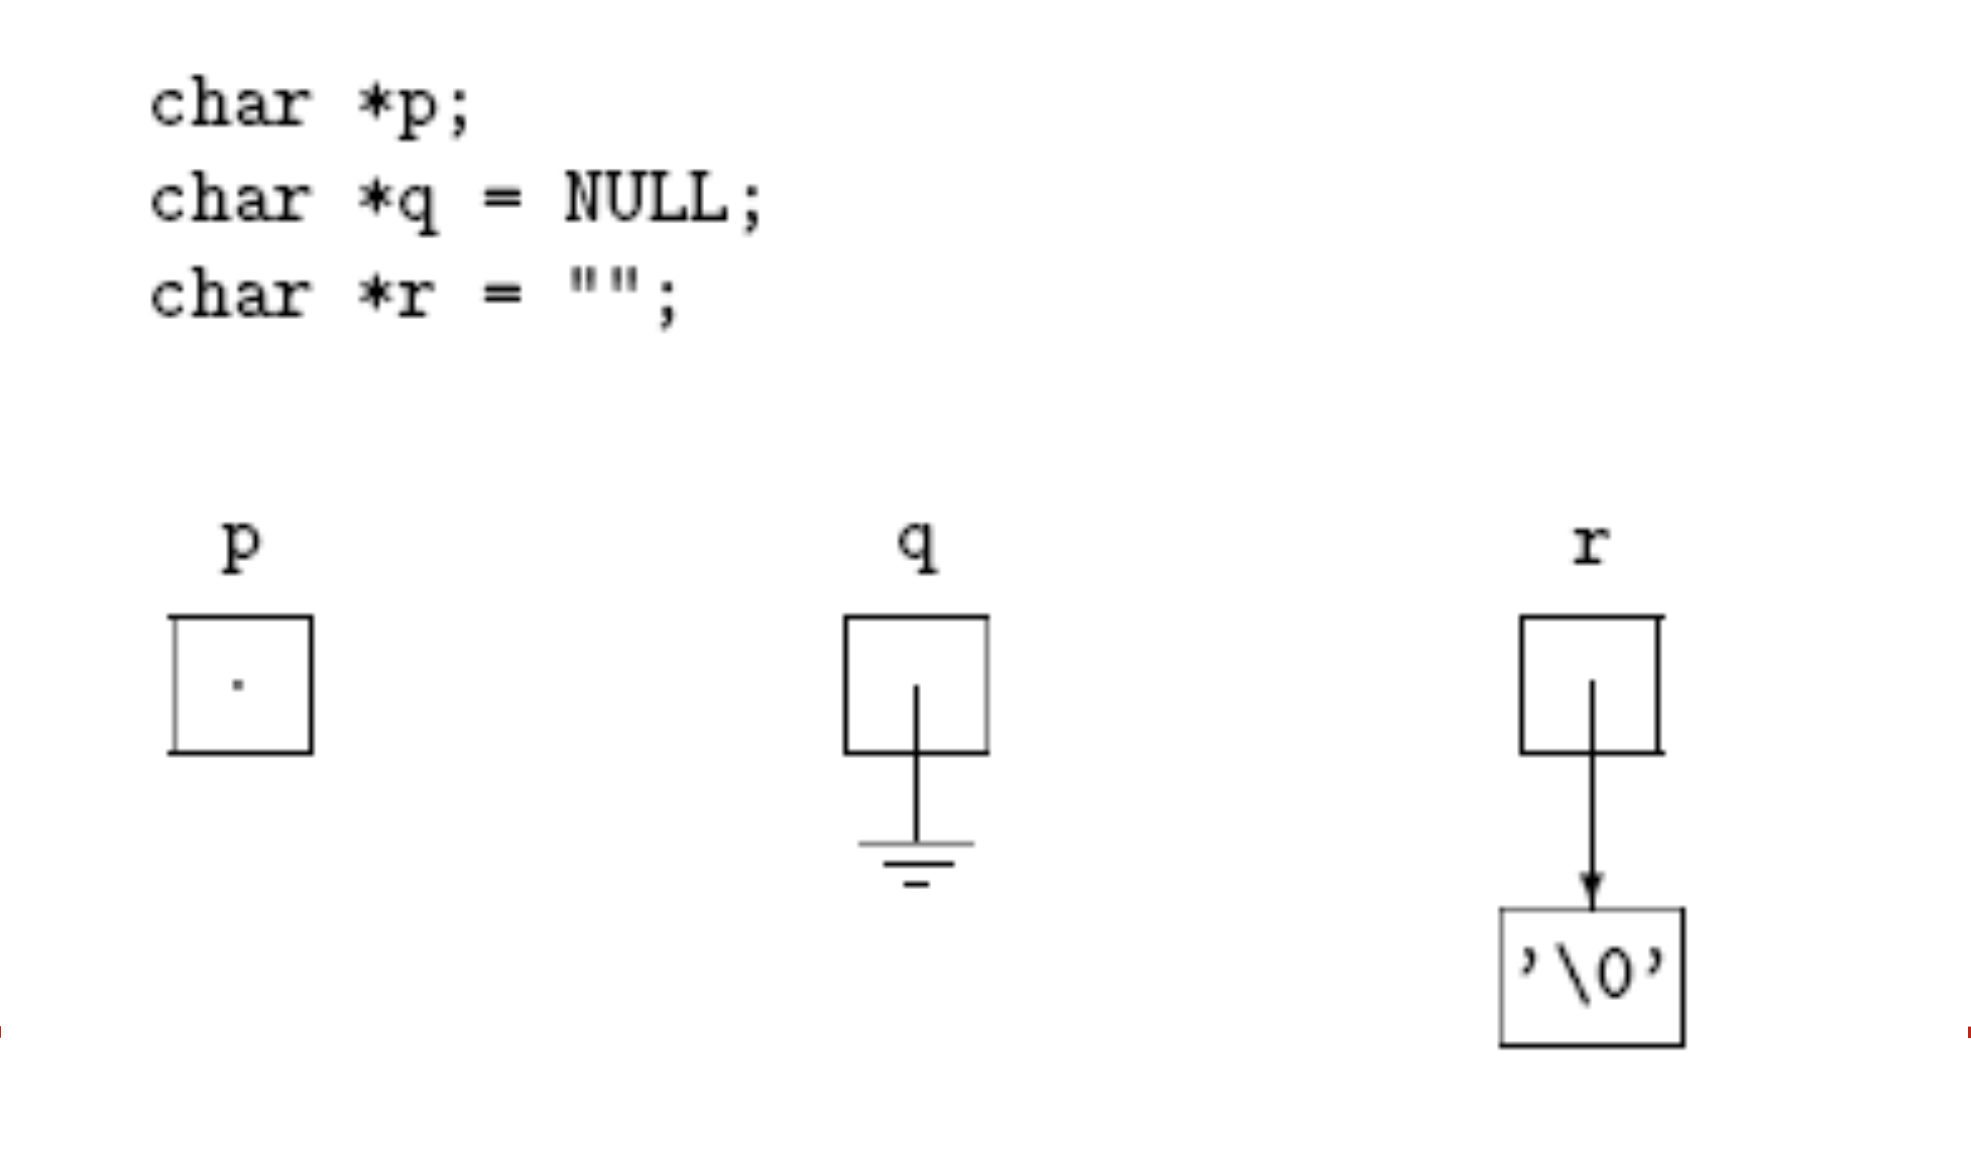
\includegraphics[height=.75\textheight]{img/null-empty-string.png}
    \end{figure}
  \end{itemize}
\end{frame}

\begin{frame}[fragile]
  \frametitle{More String Functions}
  \begin{itemize}
    \item
      char * strchr( <span class="hl-orange">const char *s</span>,
      <span class="hl-green">char c</span>
      )
    \begin{itemize}
      \item
        Return the <span class="hl-cyan">pointer</span> to the first
        occurrence of <span class="hl-green">c</span> in
        <span class="hl-orange">s</span> or
        <span class="hl-yellow">NULL</span>

      \begin{minted}[bgcolor=Black]{c}
char *s="ABZDEZFZ";
char *pc = strchr(s, 'Z');
printf("First index of Z = %d", (pc - s));

First index of Z = 2
      \end{minted}
    \end{itemize}
  \end{itemize}
\end{frame}

\begin{frame}[fragile]
  \begin{itemize}
    \item
      char * strstr( <span class="hl-orange">const char *s1</span>,
      <span class="hl-green">const char *s2</span>
      )

    \begin{itemize}
      \item
        Return <span class="hl-cyan">pointer</span> to the first occurrence of
        <span class="hl-green">s2</span> in
        <span class="hl-orange">s1</span> or
        <span class="hl-yellow">NULL</span>

      \begin{minted}[bgcolor=Black]{c}
char *s="ABCDxyEFxyGH";
char *pc = strstr(s, "xy");
printf("First index of xy = %d", (pc - s));

First index of xy = 4
      \end{minted}
    \end{itemize}
  \end{itemize}
\end{frame}

\begin{frame}[fragile]
  \begin{itemize}
    \item
      char * strdup(
      <span class="hl-orange">const char *s1</span>
      )

    \begin{itemize}
      \item
        Returns <span class="hl-cyan">a pointer</span> to a null-terminated
        byte string, which is a duplicate of the string pointed to by
        <span class="hl-orange">s1</span>.

      \item
        The returned pointer must be passed to free to avoid a memory leak.

      \item More on free/malloc later
      \begin{minted}[bgcolor=Black]{c}
char *src = "Hello World";
char *dst = NULL;

dst = strdup(src);

printf("Destination: %s\n", dst);
dst[0] = 'h'; // there is no compile error 🕺
printf("Destination: %s\n", dst);

free(dst);
      \end{minted}
    \end{itemize}
  \end{itemize}
\end{frame}

\begin{frame}[fragile]
  \frametitle{Compare n Digits after decimal point of Two Double Number}
  \begin{minted}[bgcolor=Black]{c}
#include <stdio.h>
#include <string.h>

int check_equal(double d1, double d2, int n) {
  int dot_index1, dot_index2;
  int search_size;
  char s1[50], s2[50];

  sprintf(s1, "%0.*lf", n, d1);
  sprintf(s2, "%0.*lf", n, d2);

  dot_index1 = strchr(s1, '.') - s1;
  dot_index2 = strchr(s2, '.') - s2;

  if(dot_index1 != dot_index2)
    return 0;

  search_size = dot_index1 + n + 1;
  if(strncmp(s1, s2, search_size) == 0)
    return 1;
  else
    return 0;
}

int main(void) {
  int n;
  double d1, d2;

  printf("Enter numbers d1 and d2: ");
  scanf("%lf %lf", &d1, &d2);

  printf("Enter n: ");
  scanf("%d", &n);

  if(check_equal(d1, d2, n))
    printf("Are equal\n");
  else
    printf("Are Not equal\n");

  return 0;
}
  \end{minted}
\end{frame}

\begin{frame}[fragile]
  \frametitle{String Tokenizer}
  \begin{minted}[bgcolor=Black]{c}
#include <stdio.h>
#include <string.h>

int tokenizer(const char *s, const char *token, char result[][100]){
  int result_index = 0;
  char *index;

  // s = hello
  // token = ll
  // hello
  //   ^
  //   |
  //   index
  // index - s = 2 => len
  //
  // hello
  //     ^
  //     |
  //     index + strlen(token)
  while((index = strstr(s, token)) != NULL){
    int len = index - s;
    if(len > 0){
      strncpy(result[result_index], s, len);
      result[result_index][len] = '\0';
      result_index++;
    }
    s = index + strlen(token);
  }

  if(strlen(s) > 0){
    strcpy(result[result_index], s);
    result_index++;
  }

  return result_index;
}

int main(void){
  char *s = "a123bb123ccc123dddd123eeeee123fffffffffff123";
  char *token = "123";
  char res[10][100];
  int num = tokenizer(s, token, res);

  int i;
  for(i = 0; i < num; i++)
     printf("Token %d = %s\n", i, res[i]);
  return 0;
}
  \end{minted}
\end{frame}

\section{Pointer to Pointer \& Pointer to Function}

\begin{frame}[fragile]
  \frametitle{Pointer to Pointer}
  \begin{itemize}
    \item Pointer is a variable
    \begin{itemize}
      \item Has a value: address of other value
      \item Has an address
    \end{itemize}
    \item Pointer to pointer
    \begin{itemize}
      \item Saving the address of a pointer in another pointer
    \end{itemize}
    \begin{minted}[bgcolor=Black]{c}
int i, j, *pi, *pj;
int **ppi;
pi = &i;
ppi = &pi;
j = **ppi;
pj = *ppi;
    \end{minted}
  \end{itemize}
\end{frame}

\begin{frame}[fragile]
  \frametitle{Pointer to Pointer: Example}
  \begin{minted}[bgcolor=Black]{c}
int i = 10, j = 20, k = 30;
int *pi, *pj, **ppi;

pi = &i;
pj = &j;
ppi = &pi;

printf("%d\n", *pi); // 10
printf("%d\n", **ppi); // 10
ppi = &pj;
**ppi = 100;
printf("%d\n", j); // 100
*ppi = &k;
printf("%d\n", *pj); // 30
  \end{minted}
\end{frame}

\begin{frame}
  \frametitle{Pointer to functions}
  \begin{itemize}
    \item Functions are stored in memory
    \begin{itemize}
      \item Each function has its own address
    \end{itemize}
    \item We can have pointer to function
    \begin{itemize}
      \item A pointer that store the address of a function
    \end{itemize}
    <p>
      <span class="hl-orange"><type></span> (
      <span class="hl-green">*<identifier></span>)(
      <span class="hl-cyan"><type1></span>,
      <span class="hl-cyan"><type2></span>, ...)
    </p>
    <p>
      <span class="hl-orange">int</span> (<span class="hl-green">*pf</span>)(
      <span class="hl-cyan">char</span>, <span class="hl-cyan">float</span>)
    </p>
    <p>
      <span class="hl-green">pf</span> is a pointer to a function that the
      function return <span class="hl-orange">int</span> and its inputs are
      <span class="hl-cyan">char</span> and
      <span class="hl-cyan">float</span>
    </p>
  \end{itemize}
\end{frame}

\begin{frame}[fragile]
  \frametitle{Example}
  \begin{minted}[bgcolor=Black]{c}
int f1(int x, char c){
  printf("This is f1: x = %d, c = %c\n", x, c);
  return 0;
}

int f2(int n, char m){
  printf("This is f2: n = %d, m = %c\n", n, m);
  return 0;
}

int main(void){
  int (*f)(int, char);
  f = f1; // or f = &f1;
  (*f)(10, 'a'); // This is f1: x = 10, c = a
  f = f2; // or f = &f2
  (*f)(100, 'z'); // This is f2: n = 100, m = z
  return 0;
}
  \end{minted}
\end{frame}

\begin{frame}[fragile]
  \frametitle{Pointer to function: Example 1}
  \begin{itemize}
    \item Why?
    \begin{itemize}
      \item To develop general functions
      \begin{itemize}
        \item To change function operation in run-time
      \end{itemize}
    \end{itemize}
    \item Example: atexit
    \begin{minted}[bgcolor=Black]{c}
#include <stdlib.h>

int atexit(void (*function)(void));
    \end{minted}
    \begin{itemize}
      \item To do a function, when the program is terminated
      \begin{itemize}
        \item Normal termination
      \end{itemize}
    \end{itemize}
  \end{itemize}
\end{frame}

\begin{frame}[fragile]
  \begin{minted}[bgcolor=Black]{c}
#include <stdio.h>
#include <stdlib.h>

void good_bye(void) {
  printf("Goooodddd Byeee :-)\n");
}

int main(void){
  int i;
  atexit(good_bye);
  printf("Enter an int: ");
  scanf("%d", &i);

  if (i < 0){
    printf("No negative\n");
    return 0;
  }
  if (i > 7){
    printf("No more than 7\n");
    return 0;
  }
  if (i % 2 == 0)
    printf("Go to class \n");
  else
    printf("Do the homework \n");
  return 0;
}
  \end{minted}
\end{frame}

\begin{frame}[fragile]
  \frametitle{Pointer to function: Example 2}
  \begin{itemize}
    \item Why?
    \begin{itemize}
      \item To develop general functions
      \begin{itemize}
        \item To change function operation in run-time
      \end{itemize}
      \item Example: qsort function in <stdlib.h>
      \begin{minted}[bgcolor=Black]{c}
void qsort(void *arr, int num, int element_size, int (*compare)(void *, void *))
      \end{minted}
      \item
        To sort array <span class="hl-orange">arr</span> with
        <span class="hl-green">num</span> elements of size
        <span class="hl-cyan">element\_size</span>. The order between elements is
        specified by the <span class="hl-red">compare</span> function
    \end{itemize}
  \end{itemize}
\end{frame}

\begin{frame}[fragile]
  \begin{minted}[bgcolor=Black]{c}
#include <stdio.h>
#include <stdlib.h>

int int_cmp_asc(const void *i1, const void *i2) {
  int a = *((int *)i1);
  int b = *((int *)i2);
  return (a > b) ? 1 : (a == b) ? 0 : -1;
}

int int_cmp_dsc(const void *i1, const void *i2) {
  int a = *((int *)i1);
  int b = *((int *)i2);
  return (a > b) ? -1 : (a == b) ? 0 : 1;
}

int main(void) {
  int i;
  int arr[] = {1, 7, 3, 11, 9};

  qsort(arr, 5, sizeof(int), int_cmp_asc);
  for(i = 0; i < 5; i++)
      printf("%d \n", arr[i]);

  qsort(arr, 5, sizeof(int), int_cmp_dsc);
  for(i = 0; i < 5; i++)
      printf("%d \n", arr[i]);

  return 0;
}
  \end{minted}
\end{frame}

\begin{frame}[fragile]
  \frametitle{Sort Names with qsort}
  \begin{minted}[bgcolor=Black]{c}
#include <stdio.h>
#include <string.h>
#include <stdlib.h>

int name_cmp(const void *e1, const void *e2) {
  char **a = (char**) e1;
  char **b = (char**) e2;

  return strcmp(*a, *b);
}

int main() {
  char *names[] = { "Parham", "Ali", "Saman", "Hesam" };

  for (int i = 0; i < 4; i++) {
    printf("[%d]: %s\n", i, names[i]);
  }

  printf("--\n");
  qsort(names, 4, sizeof(char *), name_cmp);
  printf("--\n");

  for (int i = 0; i < 4; i++) {
    printf("[%d]: %s\n", i, names[i]);
  }
}
  \end{minted}
\end{frame}

\section{Dynamic memory allocation}

\begin{frame}
  \frametitle{Dynamic Memory Allocation}
  \begin{itemize}
    \item Until now
    \begin{itemize}
      \item
        We define variables:
        \mint{c}|int i; int a[200]; int x[n]|

      \item
        Memory is allocated for the variables
        <span class="hl-violet">when the scope starts</span>

      \item
        Allocated memory is released
        <span class="hl-yellow">when the scope finishes</span>

    \end{itemize}
    \item
      We <span class="hl-cyan">cannot change</span> the size of the allocated
      memories

    \begin{itemize}
      \item We cannot change the size of array
    \end{itemize}
    \item These variables are in <span class="hl-orange">stack</span>
    \item
      We want to see how to allocate memory in
      <span class="hl-green">heap</span>

  \end{itemize}
\end{frame}

\begin{frame}
  \frametitle{Heap}
  \begin{itemize}
    \item Memory is compose of a few logical sections
    \begin{itemize}
      \item
        Stack is one of the logical sections that is used for function calls

      \item All automatic variables are allocated in stack
      \begin{itemize}
        \item Stack is managed by operating system
        \item Created by function call and destroyed when function ends
      \end{itemize}
    \end{itemize}
    \item Another logical section is <span class="hl-yellow">Heap</span>
    \begin{itemize}
      \item
        Heap is used for <span class="hl-green">dynamic memory allocation</span>

      \item
        Heap is managed <span class="hl-orange">by programmer</span> (at least
        in C)

      \item Memory allocation functions \& the Free function
    \end{itemize}
  \end{itemize}
\end{frame}

\begin{frame}[fragile]
  \frametitle{Dynamic Memory Allocation (cont’d)}
  \begin{itemize}
    \item Memory allocation by <span class="hl-orange">calloc</span>
    \begin{minted}[bgcolor=Black]{c}
#include <stdlib.h>
void * calloc(int num, int size);
    \end{minted}
    \item
      <span class="hl-green">void *</span> is generic pointer, it can be
      converted to every pointer type

    \item Initializes allocated memory to zero
    \item If memory is not available calloc returns \mintinline{c}|NULL|
  \end{itemize}
\end{frame}

\begin{frame}[fragile]
  \frametitle{Dynamic Memory Allocation (cont’d)}
  \begin{itemize}
    \item Memory allocation by <span class="hl-orange">malloc</span>
    \begin{minted}[bgcolor=Black]{c}
#include <stdlib.h>
void * malloc(int size);
    \end{minted}
    \item
      <span class="hl-green">void *</span> is generic pointer, it can be
      converted to every pointer type

    \item If memory is not available malloc returns \mintinline{c}|NULL|
  \end{itemize}
\end{frame}

\begin{frame}[fragile]
  \frametitle{Dynamic Memory Allocation: Example}
  \begin{minted}[bgcolor=Black]{c}
int *pi;
/* allocate memory, convert it to int * (it is not mandatory) */
pi = (int *) malloc(sizeof(int));
if (pi == NULL){
  printf("cannot allocate\n");
  return -1;
}

double *pd;
pd = calloc(1,sizeof(double));
  \end{minted}
\end{frame}

\begin{frame}[fragile]
  \frametitle{Free}
  \begin{itemize}
    \item
      In static memory allocation, memory is freed when block/scope is finished

    \item
      In dynamic memory allocation,
      \textbf{\color{Orange} we must free} the allocated memory

    \begin{minted}[bgcolor=Black]{c}
int *pi;
pi = malloc(sizeof(int));
if (pi != NULL)
  free(pi);
    \end{minted}
  \end{itemize}
\end{frame}

\begin{frame}[fragile]
  \frametitle{1 x N Array}
  \begin{minted}[bgcolor=Black]{c}
#include <stdio.h>
#include <stdlib.h>

int main(void){
  int i, n;
  int *arr;

  printf("Enter n: ");
  scanf("%d", &n);

  arr = calloc(n, sizeof(int));
  if (arr == NULL){
    printf("cannot allocate memory\n");
    exit(-1);
  }

  for(i = 0; i < n; i++)
    /* do you work here */
    arr[i] = i;

  for(i = 0; i < n; i++)
    printf("%d\n", arr[i]);

  free(arr);
  return 0;
}
  \end{minted}
\end{frame}

\begin{frame}[fragile]
  \frametitle{N x M Array}
  \begin{minted}[bgcolor=Black]{c}
#include <stdio.h>
#include <stdlib.h>

int main(void){
  int i, j, n, m;
  int **arr;

  printf("Enter n, m: ");
  scanf("%d%d", &n, &m);

  arr = malloc(n * sizeof(int *));

  for(i = 0; i < n; i++)
    arr[i] = malloc(m * sizeof(int));

  for(i = 0; i < n; i++)
    for(j = 0; j < m; j++)
      arr[i][j] = i * j;

  for(i = 0; i < n; i++)
      free(arr[i]);

  free(arr);
  return 0;
}
  \end{minted}
\end{frame}

\begin{frame}
  \frametitle{BONUS 💯}
  \begin{block}{}
    Write a code that allocates a 2-dimensional array that each of its rows has
    a different number of columns.
  \end{block}
  \begin{block}{}
    Send your solutions to
    \textit{\color{Orange} parham.alvani@gmai.com} with your student ID.
  \end{block}
  \begin{table}
  \begin{tabular}{*{8}{c}}
    \toprule
      1 &
      3 &
      7 &
      3 &
      \multicolumn{4}{c}{} \\
    \midrule
      7 &
      8 &
      \multicolumn{6}{c}{} \\
    \midrule
      2 &
      0 &
      0 &
      2 &
      1 &
      9 &
      9 &
      5 \\
    \bottomrule
  \end{tabular}
  \end{table}
\end{frame}

\begin{frame}
  \frametitle{Reallocation}
  \begin{itemize}
    \item If we need to change the size of allocated memory
    \begin{itemize}
      \item Expand or Shrink it
    \end{itemize}
    \mint{c}|void * realloc(void *p, int newsize);|
    \item
      Allocate <span class="hl-orange">newsize</span> bytes for pointer
      <span class="hl-green">p</span>

    \item Previous data of <span class="hl-green">p</span> does not change
    \item
      <span class="hl-cyan">UPDATE</span> <span class="hl-green">p</span> with
      its returned address

  \end{itemize}
\end{frame}

\begin{frame}[fragile]
  \frametitle{Reallocation: Example}
  \begin{minted}[bgcolor=Black]{c}
int *p;
p = calloc(2, sizeof(int));

printf("%d\n", *p); // 0
*p = 500;

printf("%d\n", *(p+1)); // 0
*(p + 1) = 100;

p = realloc(p, sizeof(int) * 4);

printf("%d\n", *p); // 500
p++;

printf("%d\n", *p); // 100
p++;

printf("%d\n", *p); // ?
p++;

printf("%d\n", *p); // ?
  \end{minted}
\end{frame}

\section{Common Bugs}

\begin{frame}[fragile]
  \frametitle{Common Bugs}
  \begin{itemize}
    \item
      Be {\color{Orange} very very} careful about pointers
    \begin{itemize}
      \item Invalid type of value assigned to pointer
      \begin{minted}[bgcolor=Black]{c}
int i, *pi = &i;
*pi = 29.090; // No warning!!!
      \end{minted}
      \item Invalid usage of pointers
      \begin{minted}[bgcolor=Black]{c}
int *pi, i;
pi = i;
i = pi;
      \end{minted}
    \end{itemize}
  \end{itemize}
\end{frame}

\begin{frame}[fragile]
  \begin{itemize}
    \item We cannot change constant string
    \begin{minted}[bgcolor=Black]{c}
char *s = "abc";
*(s + 1) = 'z'; // Runtime Error
    \end{minted}
  \end{itemize}
\end{frame}

\begin{frame}
  \frametitle{Legends}
  \begin{figure}
    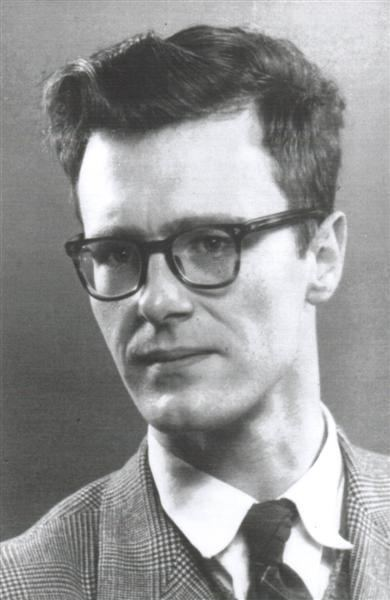
\includegraphics[height=.75\textheight]{./img/dijkstra.jpg}
  \end{figure}
  \pause%
  \centering
  \color{Violet} Edsger W. Dijkstra
\end{frame}

\begin{frame}
  \frametitle{Legends}
  \begin{itemize}
    \item
      Program testing can be used to show the presence of bugs, but never to
      show their absence!
    \item
      Dijkstra's algorithm is an algorithm for finding the shortest paths
      between nodes in a graph
  \end{itemize}
\end{frame}

\end{document}
